\fenicschapter{Instant: just-in-time compilation of C/C++ in Python}
              {Instant: just-in-time compilation of C/C++ in Python}
              {Ilmar M. Wilbers, Kent-Andre Mardal and Martin S. Aln{\ae}s}
              {wilbers}

Instant is a small Python module for just-in-time compilation
(JIT)\index{JIT} (or inlining) of C/C++ code.  Instant accepts plain
C/C++ and is therefore conveniently combined with the code generating
tools in DOLFIN, FFC, and SFC.

\section{Brief overview of Instant and its role in FEniCS}

In FEniCS, FFC and SFC are form compilers that generate UFC compliant C++
code based on the language UFL.  Within FFC and SFC, Instant is used to
JIT-compile the C++ code to a Python module.  Similarly, Instant is used
in DOLFIN to JIT-compile \emp{Expression}s and \emp{SubDomain}s.  See the
Chapters~\ref{chap:alnes-3}, \ref{chap:logg-1} and~\ref{chap:mardal-2}
for more information on these topics.

<<<<<<< TREE
Instant relies on \citet{www:swig,Beazley2006} for the generation of
=======
Instant relies on \citet{www:swig} for the generation of
>>>>>>> MERGE-SOURCE
wrapper code needed for making the C/C++ code usable from Python.  The
code to be inlined, in addition to the wrapper code, is then compiled
into a Python extension module (a shared library with functionality as
specified by the Python C-API) by using Distutils or CMake. To check
whether the C/C++ code has changed since the last execution, Instant
computes the SHA1 sum~\citep{HansenWollman} of the code and compares
it to the SHA1 checksum of the code used in the previous
execution. Finally, Instant has implemented a set of
SWIG \index{typemaps}typemaps, allowing the user to transfer NumPy
arrays between the Python code and the C/C++ code.

\section{Examples}

\label{wilbers:sec:examples}
\subsection{Hello world}
Our first example demonstrates the usage of Instant in a very simple case:
\begin{python}
from instant import inline
c_code = r'''
double add(double a, double b)
{
  printf("Hello world! C function add is being called...\n");
  return a+b;
}'''
add_func = inline(c_code)
sum = add_func(3, 4.5)
print 'The sum of 3 and 4.5 is', sum
\end{python}
When run, this script produces the following output:
\begin{progoutput}
 > python ex1.py
--- Instant: compiling ---
Hello world! C function add is being called...
The sum of 3 and 4.5 is 7.5
\end{progoutput}
Here Instant will wrap the C-function \emp{add} into a Python
extension module by using SWIG and Distutils.  The inlined function is
written in standard C. SWIG supports almost all of C and C++,
including classes and templates.  The first time the Python script is
run, it will use a few second to compile the C code.  The next time,
however, the compilation is omitted, given that no changes have been
made to the C source code.

%Note that a raw string is used in this example, to avoid Python
%interpreting escape sequences such as
%'\verb@\@\emp{n}'. Alternatively, special characters can be escaped
%using a backslash.

Although Instant notifies the user when it is compiling, it might
sometimes be necessary, e.g. when debugging, to see the details of the
Instant internals. We can do this by setting the logging level before
calling any other Instant functions:
\begin{python}
from instant import output
output.set_logging_level('DEBUG')
\end{python}
%The intrinsic Python module \emp{logging} is used. First,
%the \emp{build\_\-function} arguments are displayed, whereafter the
%different steps performed by Instant are shown in detail, e.g whether
%the module is found in cache and the arguments to the Distutils file
%when building the module.  This example can be found in the
%file \emp{examples/ex1.py}.

\subsection{NumPy arrays}

One basic problem with wrapping C and C++ code is how to handle
dynamically allocated arrays. Arrays allocated dynamically are
typically represented in C/C++ by a pointer to the first element of an
array and a separate integer variable holding the array size. In
Python the array variable is itself an object containing the data
array, array size, type information etc.  SWIG provides typemaps to
specify mappings between Python and C/C++ types. We will not go into
details on typemaps in this chapter, but the reader should be aware
that it is a powerful tool that may greatly enhance your code, but
also lead to mysterious bugs when used wrongly. Typemaps are discussed
in Chapter~\ref{chap:mardal-2} and at length in the SWIG
documentation.  In this chapter, it is sufficient to illustrate how to
deal with arrays in Instant using the NumPy module.

To illustrate the use of NumPy arrays with Instant, we introduce a
solver for an ordinary differential equation (ODE) modeling blood
pressure by using a \index{Windkessel model}Windkessel model. The ODE
is as follows:
\begin{eqnarray}
\frac{d}{dt}p(t) &=& B Q(t) - A p(t), \quad t \in (0,1), \\
p(0) &=& p0.
\end{eqnarray}
Here $p(t)$ is the blood pressure, $Q(t)$ is the volume flux of blood,
while $A$ and $B$ are real numbers representing resistance and compliance, respectively.
An explicit scheme is:
\begin{eqnarray}
p_i &=& p_{i-1} + \Delta t (B Q_i - A p_{i-1}), \quad \mbox{for}\quad i=1,\ldots,N-1,  \\
p_0 &=& p0.
\end{eqnarray}
The scheme can be implemented in Python as follows using NumPy arrays:
\begin{python}
def time_loop_py(p, Q, A, B, dt, N, p0):
    p[0] = p0
    for i in range(1, N):
        p[i] = p[i-1] + dt*(B*Q[i] - A*p[i-1])
\end{python}
The corresponding C code is:
\begin{c++}
void time_loop_c(int n, double* p,
                 int m, double* Q,
                 double A, double B,
                 double dt, int N, double p0)
{
    if ( n != m || N != m )
    {
        printf("n, m and N should be equal\n");
        return;
    }

    p[0] = p0;
    for (int i=1; i<n; i++)
    {
        p[i] = p[i-1] + dt*(B*Q[i] - A*p[i-1]);
    }
}
\end{c++}
In this example, \emp{(int n, double* p)} represents an array of
doubles with length $n$. However, this can not be determined by the
function signature:
\begin{c++}
void time_loop_c(int n, double* p, int m, double* Q, ...)
\end{c++}
For example, \emp{double* p} may be an array of length $m$ or it may simply be
output. In Instant you must therefore specify what the arrays are:
\begin{python}
time_loop_c = inline_with_numpy(c_code,
                                arrays = [['n', 'p'],
                                          ['m', 'Q']])
\end{python}
Here, we tell Instant that \emp{(int n, double* p)} and
\emp{(int m, double* Q)} are NumPy arrays (and Instant then generates the
proper typemaps).
We may then call the \emp{time\_\-loop}
function as follows:
\begin{python}
time_loop_c(p, Q, 1.0, 1.0, 1.0/(N-1), N, 1.0)
\end{python}

In Table \ref{wilbers:fig:speed-up} we compare the above mentioned
code with pure C code, pure Python, and NumPy.  We obtain a speed-up
of about a factor 350 when compared with NumPy, using $10^5$ time
steps. The performance of the code using Instant is actually the same
as a pure C program.  The comparison between NumPy and Instant may not
be completely fair. NumPy is primarily intended for algorithms that
can be vectorized, which is not the case with ODEs. In fact, utilizing
pure Python lists instead of NumPy arrays, reduces the speed-up to a
factor 65. For code that can be vectorized, the speed-up is about one
order of magnitude, when using Instant instead of
NumPy~\citep{WilbersLangtangenOdegaard2009}.  The result of solving the ODE
can be seen in Figure
\ref{wilbers:fig:fig1}.

\begin{figure}
\begin{center}
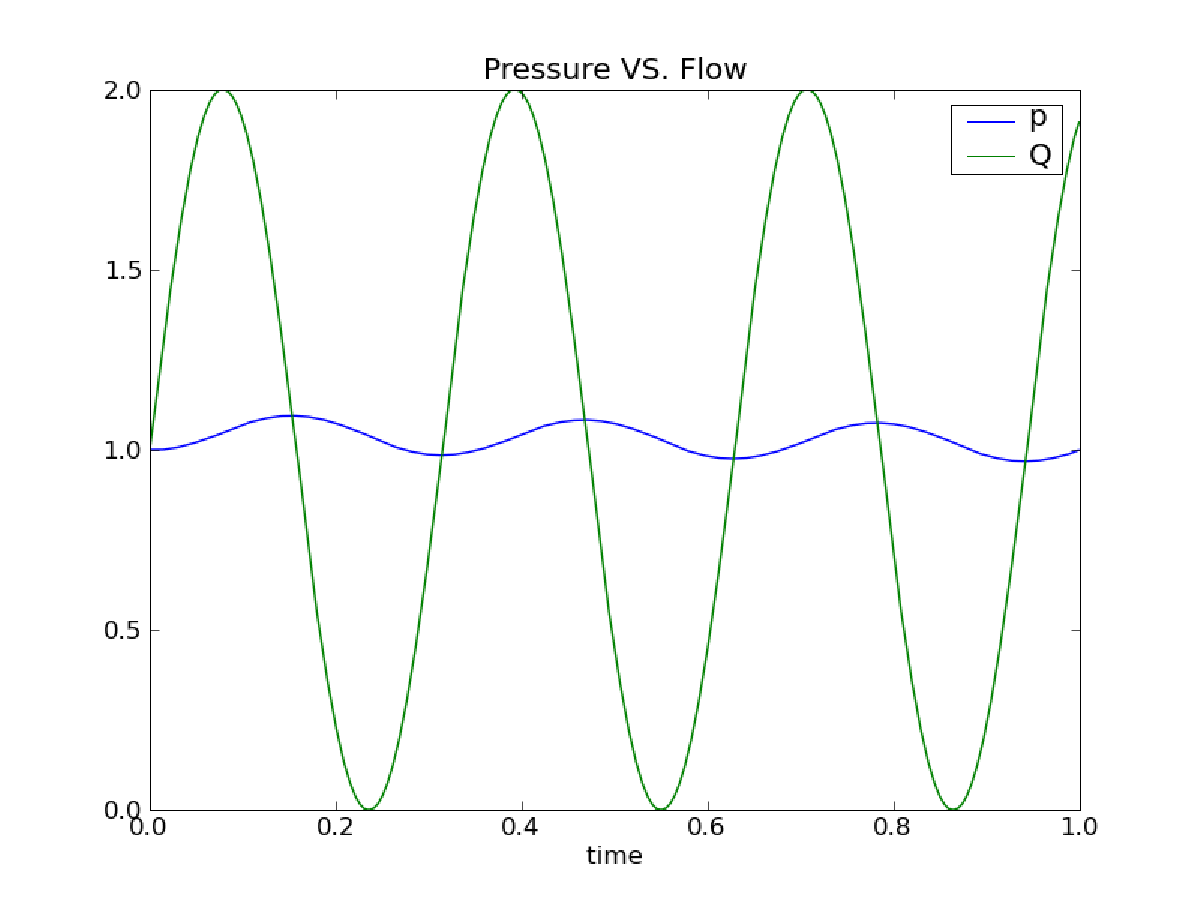
\includegraphics[width=100mm]{chapters/wilbers/pdf/pressure_plot.pdf}
\caption{Plot of pressure and blood volume flux computed by solving the Windkessel model.}
\label{wilbers:fig:fig1}
\end{center}
\end{figure}

\begin{table}
\begin{center}
\begin{tabular}{|l|c|c|c|c|c|} \hline
N                     & $10^2$     & $10^3$ & $10^4$ &  $10^5$ &  $10^6$ \\ \hline
CPU time with NumPy   & 3.9e-4  & 3.9e-3 & 3.8e-2 & 3.8e-1 & 3.8     \\ \hline
CPU time with Python  & 0.7e-4  & 0.7e-3 & 0.7e-2 & 0.7e-1 & 0.7     \\ \hline
CPU time with Instant & 5.0e-6  & 1.4e-5 & 1.0e-4 & 1.0e-3 & 1.1e-2  \\ \hline
CPU time with C       & 4.0e-6  & 1.1e-5 & 1.0e-4 & 1.0e-3 & 1.1e-2  \\ \hline
\end{tabular}
\caption{CPU times (in seconds) for solving the ODEs from the  Windkessel model using different implementations.}
\label{wilbers:fig:speed-up}
\end{center}
\end{table}
The complete code for this example can be found in \emp{ex2.py}.


\subsection{NumPy arrays and OpenMP}

It is easy to speed up code on parallel computers with OpenMP. In the
following code preprocessor directives like '\emp{\#pragma
omp \ldots}' are OpenMP directives and OpenMP functions always start
with \emp{omp}.  In this example, we want to solve a standard
2-dimensional wave equation in a heterogeneous medium with local wave
velocity $k$:
\begin{equation}
\frac{\partial^2u}{\partial t^2} = \nabla \cdot [k\nabla u]\, .
\end{equation}
We set the boundary condition to $u = 0$ for the whole boundary of a
rectangular domain $\Omega = (0,1) \times (0,1)$. Further, $u$ has the initial
value $I(x,y)$ at $t = 0$ while $\partial u/ \partial t = 0$.
We solve the wave equation using the following finite difference scheme:
\begin{align}
u_{i,j}^l =
&\left(\frac{\Delta t}{\Delta x}\right)^2
[k_{i+\frac{1}{2},j}(u_{i+1,j} - u_{i,j}) - k_{i-\frac{1}{2},j}(u_{i,j} - u_{i-1,j})]^{l-1}\notag\\
+&\left(\frac{\Delta t}{\Delta y}\right)^2
[k_{i,j+\frac{1}{2}}(u_{i,j+1} - u_{i,j}) - k_{i,j-\frac{1}{2}}(u_{i,j} - u_{i,j-1})]^{l-1}.
\end{align}\label{u}
Here, $u_{i,j}^l$ represents $u$ at the grid point $x_i$ and $y_j$ at
time level $t_l$, where
\begin{align}
x_i &= i\Delta x, i = 0, \ldots, n\\
y_i &= j\Delta y, j = 0, \ldots, m\textrm{ and}\\
t_l &= l\Delta t,
\end{align}
Also, $k_{i+\frac{1}{2},j}$ is short for $k(x_{i+\frac{1}{2}},y_j)$.

The code for calculating the next time step using OpenMP looks like:
\begin{c++}
void stencil(double dt, double dx, double dy,
             int ux, int uy, double* u,
             int umx, int umy, double* um,
             int kx, int ky, double* k,
             int upn, double* up){
#define index(u, i, j) u[(i)*m + (j)]
  int i=0, j=0, m = ux, n = uy;
  double hx, hy, k_c, k_ip, k_im, k_jp, k_jm;
  hx = pow(dt/dx, 2);
  hy = pow(dt/dy, 2);
  j = 0;   for (i=0; i<m; i++) index(up, i, j) = 0;
  j = n-1; for (i=0; i<m; i++) index(up, i, j) = 0;
  i = 0;   for (j=0; j<n; j++) index(up, i, j) = 0;
  i = m-1; for (j=0; j<n; j++) index(up, i, j) = 0;
  #pragma omp for
  for (i=1; i<m-1; i++){
    for (j=1; j<n-1; j++){
      k_c = index(k, i, j);
      k_ip = 0.5*(k_c + index(k, i+1, j));
      k_im = 0.5*(k_c + index(k, i-1, j));
      k_jp = 0.5*(k_c + index(k, i, j+1));
      k_jm = 0.5*(k_c + index(k, i, j-1));
      index(up, i, j) = 2*index(u, i, j) - index(um, i, j) +
        hx*(k_ip*(index(u, i+1, j) - index(u, i, j)) -
             k_im*(index(u, i, j) - index(u, i-1, j))) +
        hy*(k_jp*(index(u, i, j+1) - index(u, i, j)) -
            k_jm*(index(u, i, j) - index(u, i, j-1)));
    }
  }
}
\end{c++}
We also need to add the OpenMP header \emp{omp.h} and compile
with the flag \emp{-fopenmp} and link with the OpenMP shared
library, e.g. \emp{libgomp.so} for Linux (specified with \emp{-lgomp}).
This can be done as follows:
\begin{python}
instant_ext = \
  build_module(code=c_code,
               system_headers=['numpy/arrayobject.h',
                               'omp.h'],
               include_dirs=[numpy.get_include()],
               init_code='import_array();',
               cppargs=['-fopenmp'],
               lddargs=['-lgomp'],
               arrays=[['ux', 'uy', 'u'],
               ['umx', 'umy', 'um'],
               ['kx', 'ky', 'k'],
               ['upn', 'up', 'out']])
\end{python}
Note that the arguments \emp{include\_\-headers}, \emp{init\_\-code},
and the first element of \emp{system\_\-headers} could have been
omitted if we used \emp{inline\_\-module\_\-with\_\-numpy}(see below)
instead of \emp{build\_\-module}.  The complete code can be found
in \emp{ex3.py}.

In Table \ref{speed-up2} we have compared the timings of running with
different numbers of CPUs. The timings in this table are performed on
a quad-core machine with 32GB memory. We see a speed-up of factor two
when doubling the number of CPUs, but further increasing the number of
CPUs has a limited effect. We have not been able to investigate this
further, but suspect that the physical layout of the machine with two
dual cores causes this, as the two CPUs on the same core share some of
the resources.
\begin{table}
\begin{center}
\begin{tabular}{|l|c|c|} \hline
N                     & 1e+8     &2e+8 \\ \hline
CPU time with Instant 1 CPU & 0.80  & 1.59  \\ \hline
CPU time with Instant 2 CPU & 0.42  & 0.81  \\ \hline
CPU time with Instant 3 CPU & 0.37  & 0.75  \\ \hline
CPU time with Instant 4 CPU & 0.34  & 0.67  \\ \hline
\end{tabular}
\caption{CPU times (in seconds) for the implementation of the solution of a wave-equation
using Instant and OpenMP on different numbers of CPUs/threads.}
\label{speed-up2}
\end{center}
\end{table}

\section{Errors encountered when using Instant}

There are basically three different types of errors you can encounter
when using Instant.  These are: 1) errors caused by non-compilable
C/C++ code, 2) errors caused by wrong usage of SWIG, and 3) errors
related to importing the module from the cache. We will now go briefly
through these three different types of errors. Let us start by
removing a ';' in the C++ code of
\emp{ex2.py}, making the C++ compiler unable to compile the code. We will then get errors on the
following form:
\begin{progoutput}
--- Instant: compiling ---
In instant.recompile: The module did not compile,
   see '/tmp/tmpZ4M_ZO2010-11-9-08-24_instant/instant_module_dff94651124193a[...]
Traceback (most recent call last):
      File "test2.py", line 21, in <module>
          sum_func = inline_with_numpy(c_code, arrays = [['n1', 'array1']])
        File "/usr/local/lib/python2.6/dist-packages/instant/inlining.py", line 95, in inline_with_numpy
          module = build_module(**kwargs)
        File "/usr/local/lib/python2.6/dist-packages/instant/build.py", line 474, in build_module
          recompile(modulename, module_path, setup_name, new_compilation_checksum)
        File "/usr/local/lib/python2.6/dist-packages/instant/build.py", line 100, in recompile
          "compile, see '%s'" % compile_log_filename)
        File "/usr/local/lib/python2.6/dist-packages/instant/output.py", line 49, in instant_error
          raise RuntimeError(text)
      RuntimeError: In instant.recompile: The module did not compile,
      see '/tmp/tmpZ4M_ZO2010-11-9-08-24_instant/instant_module_dff946511241[...]
\end{progoutput}
The error message from the compiler is located in the file \emp{compile.log} in the temporary directory
\emp{/tmp/tmpZ4M\_ZO2010-11-9-08-24\_instant/instant\_module\_dff946511241aab327593a2d71105c5fc/}.
The compile error message will here refer to line numbers in the
wrapper code generated by SWIG.  You should still be able to locate
the C++ error, by looking at the error message in \emp{compile.log}
and the file containing the wrapper code (named \emp{*\_wrap.cxx}) in
the temporary directory.

The second type of error occurs when SWIG is not able to parse the
code. These errors are easily identified by the first line in the
error message, namely
\emp{Error: Syntax error in input(1).}
\begin{progoutput}
instant_module_815d9b7181988c1596a71b62f8a17936a77e5944.i:39: Error: Syntax error in input(1).
running build_ext
building '_instant_module_815d9b7181988c1596a71b62f8a17936a77e5944' extension
creating build
creating build/temp.linux-i686-2.6
gcc -pthread -fno-strict-aliasing -DNDEBUG -g -fwrapv -O2 -Wall -Wstrict-prototypes -fPIC
   -I/usr/lib/python2.6/dist-packages/numpy/core/include -I/usr/include/python2.6
   -c instant_module_815d9b7181988c1596a71b62f8a17936a77e5944_wrap.cxx
   -o build/temp.linux-i686-2.6/instant_module_815d9b7181988c1596a71b62f8a1[...].o -O2
gcc: instant_module_815d9b7181988c1596a71b62f8a17936a77e5944_wrap.cxx: No such file or directory
gcc: no input files
\end{progoutput}
SWIG reports that it is unable to parse the Instant generated
interface file (named \emp{*.i}) and that the problem arises at line
39.  In this case, you should have a look in the generated interface
file in the temporary directory.

Finally, Python may not be able to import the module from the
cache. There might be numerous reasons for this; the cache may be old
and incompatible with the current version of Python, the cache may be
corrupted due to disk failure, some shared libraries might be missing
from \emp{\$LD\_LIBRARY\_PATH} and so on.  Such error messages look
like:
\begin{progoutput}
In instant.import_module_directly:
Failed to import module 'instant_module_4b41549bc6282877d3f97d54ef664d4' from '/home/kent-and/.instant/cache'.
Traceback (most recent call last):
  File "test2.py", line 21, in <module>
    sum_func = inline_with_numpy(c_code, arrays = [['n1', 'array1']])
  File "/usr/local/lib/python2.6/dist-packages/instant/inlining.py", line 95, in inline_with_numpy
    module = build_module(**kwargs)
  File "/usr/local/lib/python2.6/dist-packages/instant/build.py", line 383, in build_module
    module = check_disk_cache(modulename, cache_dir, moduleids)
  File "/usr/local/lib/python2.6/dist-packages/instant/cache.py", line 121, in check_disk_cache
    module = import_and_cache_module(path, modulename, moduleids)
  File "/usr/local/lib/python2.6/dist-packages/instant/cache.py", line 67, in import_and_cache_module
    instant_assert(module is not None, "Failed to import module found in cache."
  File "/usr/local/lib/python2.6/dist-packages/instant/output.py", line 55, in instant_assert
    raise AssertionError(text)
\end{progoutput}
In this case it is advantageous to make a local cache, using the  \emp{cache\_dir="test\_cache"}, and go
to the local cache to find the error.

\section{Instant explained}
\label{wilbers:sec:explained}

The previous section concentrated on the usage of Instant.  In this
section we explain what Instant does.  We will again use our first
example, but we set the module name explicitly with the keyword
argument \emp{modulename} to see more clearly what happens:
\begin{python}
from instant import inline
code = r'''
double add(double a, double b)
{
  printf("Hello world! C function add is being called...\n");
  return a+b;
}'''
add_func = inline(code, modulename='ex4')
sum = add_func(3, 4.5)
print 'The sum of 3 and 4.5 is', sum
\end{python}
After running this code there is a new directory \emp{ex4} in our directory.
The contents is:
\begin{progoutput}
~/instant_doc/code$ cd ex4/
~/instant_doc/code/ex4$ ls -g
total 224
drwxr-xr-x 4 ilmarw  4096 2009-05-18 16:52 build
-rw-r--r-- 1 ilmarw   844 2009-05-18 16:52 compile.log
-rw-r--r-- 1 ilmarw   183 2009-05-18 16:52 ex4-0.0.0.egg-info
-rw-r--r-- 1 ilmarw    40 2009-05-18 16:52 ex4.checksum
-rw-r--r-- 1 ilmarw   402 2009-05-18 16:53 ex4.i
-rw-r--r-- 1 ilmarw  1866 2009-05-18 16:52 ex4.py
-rw-r--r-- 1 ilmarw  2669 2009-05-18 16:52 ex4.pyc
-rwxr-xr-x 1 ilmarw 82066 2009-05-18 16:52 _ex4.so
-rw-r--r-- 1 ilmarw 94700 2009-05-18 16:52 ex4_wrap.cxx
-rw-r--r-- 1 ilmarw    23 2009-05-18 16:53 __init__.py
-rw-r--r-- 1 ilmarw   448 2009-05-18 16:53 setup.py
\end{progoutput}
The file \emp{ex4.i} is the SWIG interface file.
Another central file is the Distutils file \emp{setup.py}, which is generated
and executed. During execution, \emp{setup.py} first runs SWIG on the interface file,
producing \emp{ex4\_wrap.cxx} and \emp{ex4.py}. The first file
is then compiled into a shared library  \emp{\_ex4.so}
(note the leading underscore). The file \emp{ex4-0.0.0.egg-info}
and the directory \emp{build} are also created by Distutils.
The output from executing the Distutils file is stored in the file
\emp{compile.log}.  Finally, a checksum file named
\emp{ex4.checksum} is generated, containing a checksum based on
the files present in the directory. The final step consists of moving
the whole directory from its temporary location to either cache or a
user-specified directory. The file \emp{\_\-\_\-init\_\-\_\-.py}
imports the module
\emp{ex4} into Python.

The script \index{\emp{instant-clean}}\emp{instant-clean} removes
compiled modules from the Instant cache, located in the directory
\emp{.instant} in the home directory of the user running it.
The script \index{\emp{instant-showcache}}\emp{instant-showcache}
shows the modules located in the Instant cache.

\subsection{Arrays and typemaps}\label{wilbers:sec:arrays}

Instant has support for converting NumPy arrays to C arrays and vice
versa. Each array specification is a list containing the names of the
variables describing that array in the C code. For a 1D array, this
means the names of the variables containing the length of the array
(an \emp{int}), and the array pointer. The array pointer can have
several types, but the default is \emp{double}. For 2D arrays we need
three strings, two for the length in each dimension, and one for the
array pointer. This following example illustrate the array
specification:
\begin{python}
arrays = [['len', 'a'],                        # a 1D array / vector
          ['len_bx', 'len_by', 'b'],           # a matrix
          ['len_cx', 'len_cy', 'len_cz', 'c']] # a 3D tensor
\end{python}
The variables names specified reflect the variable names in the C function
signature. It is important that the order of the variables in the signature is
retained for each array; that is, the signature should be:
\begin{c++}
double sum (int len_a, double*a,
	          int len_bx, int len_by, double* b,
	          int len_cx, int len_cy, int_cz, double* c)
\end{c++}
The arrays are assumed to be of type \emp{double} by default, but
several other types are supported. These types
are \emp{float}, \emp{short}, \emp{int}, \emp{long}, \emp{long
long}, \emp{unsigned short}, \emp{unsigned int}, \emp{unsigned long},
and \emp{unsigned long long}. The type can be specified by adding an
additional value to the list describing the array, e.g.
\begin{python}
arrays = [['len', 'a', 'long']]
\end{python}
It is important that there is correspondence between the type of the
NumPy array and the type in the signature of the C function. For
arrays that are changed in-place, the types have to match exactly. For
arrays that are input or output (see next section), one has to make
sure that the implicit casting is done to a type with higher
precision. For input arrays, the C type must be of the same or higher 
precision as the NumPy array, while for output arrays the NumPy array
type must be of the same or higher precision as the C array. The
NumPy type \emp{float32} corresponds to the C type \emp{float},
while \emp{float64} corresponds to \emp{double}. The NumPy
type \emp{float} is the same as \emp{float64}. For integer arrays, the
mapping between NumPy types and C types depends on your
system. Using \emp{long} as the C type will work in most cases.

Instant supports both input, output and in-place arrays.  The default
behavior is to treat the arrays as in-place arrays, provided that the
input are NumPy arrays. Python lists and sequences are converted to
NumPy arrays automatically.  The following code shows an example where
we calculate the matrix-vector multiplication $x = Ab$. The integer
matrix $A$ and double vector $b$ are marked as input, while the double
vector $x$ is output. The code can be found in: \emp{ex5.py}.
\begin{python}
from instant import inline_with_numpy
from numpy import arange, dot

c_code = '''
void dot_c(int Am, int An, long* A, int bn, int* b,
           int xn, double* x)
{
  for (int i=0; i<Am; i++)
  {
    x[i] = 0;
    for (int j=0; j<An; j++)
    {
      x[i] += A[i*Am + j]*b[j];
    }
  }
}
'''
dot_c = \
  inline_with_numpy(c_code,
                    arrays = [['Am', 'An', 'A', 'in', 'long'],
                              ['bn', 'b', 'in'],
                              ['xn', 'x', 'out']])
a = arange(9)
a.shape = (3, 3)
b = arange(3)

c = dot_c(a, b, a.shape[1])
\end{python}

Finally, it is possible to work with arrays that are more than
3-dimensional.  However, the typemaps used for this employ less error
checking, and can currently only be used for the C
type \emp{double}. The list describing the array should contain the
variable name for holding the number of dimensions, the variable name
for an integer array holding the size in each dimension, the variable
name for the array, and the argument \emp{'multi'}, indicating that it
has more than 3 dimensions. The \emp{arrays} argument could for
example be:
\begin{python}
arrays = [['m', 'mp', 'ar1', 'multi'],
          ['n', 'np', 'ar2', 'multi']]
\end{python}
In this case, the C function signature should look like:
\begin{c++}
void sum (int m, int* mp, double* ar1, int n,
          int* np, double* ar2)
\end{c++}

\subsection{Module name, signature, and cache}\label{wilbers:sec:msc}

\index{cache}\index{signatures}
The Instant cache resides in the directory \emp{.instant} in the
home directory of the user. It is possible to specify a different directory, but the
\emp{instant-clean} script will not remove these when executed.
The three keyword arguments \emp{modulename}, \emp{signature}, and
\emp{cache\_\-dir} are related. If none of them are given, the default behavior is to
create a signature from the contents of the files and arguments to the
\emp{build\_\-module} function. In this case the resulting name starts with
\emp{instant\_\-module\_\-} and is followed by a long checksum. The
resulting code is copied to the Instant cache
unless \emp{cache\_\-dir} is set to a specific directory. Note that
changing the arguments, code or compile arguments will result in a new
directory in the Instant cache.  Before compiling a module, Instant
will always check if the module is cached in either in the Instant cache or
in the current working directory.

If \emp{modulename} is used, the directory with the resulting code is
named accordingly, but not copied to the Instant cache. Instead, it is
stored in the current working directory. Any changes to the argument
or the source files will automatically result in a recompilation. The
argument \emp{cache\_\-dir} is ignored.

When \emp{signature} is given as argument, Instant uses the signature
instead of computing the checksum. The resulting directory has the
same name if signature contains less or equal to 100 characters (letters, numbers, or underscores). If this is not the case, the module name is generated
based on the checksum of this string, resulting in a module name
starting with \emp{instant\_\-module\_\-} followed by the
checksum. Because the user specifies the signature herself, changes in
the arguments or source code will not cause a recompilation.

In addition to the disk cache discussed so far, Instant also has a
memory cache. All modules used during the life-time of a program are
stored in memory for faster access. The memory cache is always checked
before the disk cache.

\subsection{Locking}

Instant provides file locking functionality for cache modules. If
multiple processes are working on the same module, race conditions
could potentially occur, where two or more processes believe the
module is missing from the cache and try to write it
simultaneously. To avoid race conditions, lock files have been
introduced. The lock files reside in the Instant cache, and locking is
only enabled for modules that should be cached; that is, where the
module name is not given explicitly as argument
to \emp{build\_\-module} or one of its wrapper functions. The first
process to reach the stage where the module is copied from its
temporary location to the Instant cache, will acquire a lock, and
other processes cannot access this module while it is being copied.

%FIXME: More about locking? How do we finish the whole thing?

\section{Instant API}

\label{wilbers:sec:api}
In this section we will describe the various Instant functions and
their arguments. The first six functions are the core Instant
functions. The function \emp{build\_\-module} is the main function,
while the five next functions are are wrappers around this
function. Finally, there are also four helper functions available,
intended for using Instant with other applications.

\subsection[build\_module]{\emp{build\_module}}

This function is the most important one in Instant, and for most applications
the only one that developers need to use (together with the wrapper functions).
The return argument is the compiled module, which
can be used directly in the calling code.

There are a number of keyword arguments, and we will explain them in detail
here. Although one of the aims of Instant is to minimize the direct
interaction with SWIG, some of the keywords require knowledge of SWIG
in order to make sense. In this way, Instant can be used both by programmers
new to the use of extension languages for Python, as well as by experienced
SWIG programmers. The keywords arguments are as follows:
\begin{itemize}
\item \emp{modulename}
  \begin{itemize}
  \item Default: \emp{None}
  \item Type: String
  \item Comment: The name you want for the module.
    If specified, the module will not be cached.
    If missing, a name will be constructed based on
    a checksum of the other arguments, and the module
    will be placed in the global cache.
  \end{itemize}
\item \emp{source\_\-directory}
  \begin{itemize}
    \item Default: '.'
    \item Type: String
    \item Comment: The directory where user supplied files reside. The files
      given in \emp{sources}, \emp{wrap\_\-headers}, and \emp{local\_\-headers}
      are expected to exist in this directory.
  \end{itemize}
\item \emp{code}
  \begin{itemize}
    \item Default: \emp{''}
    \item Type: String
    \item Comment: The C or C++ code to be compiled and wrapped.
  \end{itemize}
\item \emp{init\_\-code}
  \begin{itemize}
    \item Default: \emp{''}
    \item Type: String
    \item Comment: Code that should be executed when the Instant module is
      initialized. An
      example of initialization code is the call \emp{import\_\-array()} required for
      initialization of NumPy.
  \end{itemize}
\item \emp{additional\_\-definitions}
  \begin{itemize}
    \item Default: \emp{''}
    \item Type: String
    \item Comment: Additional definitions needed in the interface file.
      These definitions should be additional code that is not found
      elsewhere, but is needed by the wrapper code.
      These definitions should be given as triple-quoted
      strings in the case they span multiple lines, and are placed both in the
      initial block for C/C++ code (\emp{\%\{,\%\}}-block), and the main section
      of the interface file.
  \end{itemize}
\item \emp{additional\_\-declarations}
  \begin{itemize}
    \item Default: \emp{''}
    \item Type: String
    \item Comment: Additional declarations needed in the interface file.
      These declarations should be declarations of code that is found
      elsewhere, but is needed to make SWIG generate wrapper code properly.
      These declarations should be given as triple-quoted
      strings in the case they span multiple lines, and are placed in the main
      section of the interface file.
  \end{itemize}
\item \emp{sources}
  \begin{itemize}
    \item Default: \emp{[]}
    \item Type: List of strings
    \item Comment: Source files to compile and link with the module. These
      files are compiled together with the SWIG-generated wrapper file into
      the shared library file. Should reside in the directory specified in
      \emp{source\_\-directory}.
  \end{itemize}
\item \emp{wrap\_\-headers}
  \begin{itemize}
    \item Default: \emp{[]}
    \item Type: List of strings
    \item Comment: Local header files that should be wrapped by SWIG. The
      files specified will be included both in the initial block for C/C++ code
      (with a C directive) and in the main section of the interface file (with
      a SWIG directive). Should reside in the directory specified in
      \emp{source\_\-directory}.
  \end{itemize}
\item \emp{local\_\-headers}
  \begin{itemize}
    \item Default: \emp{[]}
    \item Type: List of strings
    \item Comment: Local header files required to compile the wrapped
      code. The files specified will be included in the initial block for C/C++ code
      (with a C directive). Should reside in the directory specified in
      \emp{source\_\-directory}.
  \end{itemize}
\item \emp{system\_\-headers}
  \begin{itemize}
    \item Default: \emp{[]}
    \item Type: List of strings
    \item Comment: System header files required to compile the wrapped
      code. The files specified will be included in the initial block for C/C++
      code (with a C directive).
  \end{itemize}
\item \emp{include\_\-dirs}
  \begin{itemize}
    \item Default: \emp{[]}
    \item Type: List of strings
    \item Comment: Directories to search for header files for building the
      extension module. Need to be absolute path names.
  \end{itemize}
\item \emp{library\_\-dirs}
  \begin{itemize}
    \item Default: \emp{[]}
    \item Type: List of strings
    \item Comment: Directories to search for libraries (\emp{-l}) for building
      the extension module. Need to be absolute paths.
  \end{itemize}
\item \emp{libraries}
  \begin{itemize}
    \item Default: \emp{[]}
    \item Type: List of strings
    \item Comment: Libraries needed by the Instant module. The libraries will
      be linked in from the shared object file. The initial \emp{-l} is added
      automatically.
  \end{itemize}
\item \emp{swigargs}
  \begin{itemize}
    \item Default: \emp{['-c++', '-fcompact', '-O', '-I.', '-small']}
    \item Type: List of strings
    \item Comment: Arguments to swig, e.g. \emp{['-lpointers.i']}
      to include the SWIG library \emp{pointers.i}.
  \end{itemize}
\item \emp{swig\_\-include\_\-dirs}
  \begin{itemize}
    \item Default: \emp{[]}
    \item Type: List of strings
    \item Comment: Directories to include in the \emp{swig} command.
  \end{itemize}
\item \emp{cppargs}
  \begin{itemize}
    \item Default: \emp{['-O2']}
    \item Type: List of strings
    \item Comment: Arguments to the C++ compiler (except include
      directories) e.g. \emp{['-Wall', '-fopenmp']}.
  \end{itemize}
\item \emp{lddargs}
  \begin{itemize}
    \item Default: \emp{[]}
    \item Type: List of strings
    \item Comment: Arguments to the linker, other than libraries and library
      directories, e.g. \emp{['-E', '-U']}.
  \end{itemize}
%\item \emp{object\_\-files}
%  \begin{itemize}
%    \item Default: \emp{[]}
%    \item Type: List of strings
%    \item Comment: If you want to compile the files yourself. TODO: Not yet
%      supported.
%  \end{itemize}
\item \emp{arrays}
  \begin{itemize}
    \item Default: \emp{[]}
    \item Type: List of strings
    \item Comment: A nested list describing the C arrays to be made from the NumPy arrays.
        For 1D arrays, the list should contain strings with the variable names for the length of
        the arrays and the array itself. Matrices should contain the names
        of the dimensions in the two directions as well as the name of the
        array, and 3D tensors should contain the names of the dimensions in
        the three directions in addition to the name of the array.
        If the NumPy array has more than three dimensions, the list should
        contain strings with variable names for the number of dimensions,
        the length in each dimension as a pointer, and the array itself,
        respectively.
  \end{itemize}
\item \emp{generate\_\-interface}
  \begin{itemize}
    \item Default: \emp{True}
    \item Type: Boolean
    \item Comment: Indicate whether you want to generate the interface files.
  \end{itemize}
\item \emp{generate\_\-setup}
  \begin{itemize}
    \item Default: \emp{True}
    \item Type: Boolean
    \item Comment: Indicate if you want to generate the \emp{setup.py} file.
  \end{itemize}
\item \emp{signature}
  \begin{itemize}
    \item Default: \emp{None}
    \item Type: String
    \item Comment: A signature string to identify the form instead of the
      source code. See Section \ref{wilbers:sec:msc}.
  \end{itemize}
\item \emp{cache\_\-dir}
  \begin{itemize}
    \item Default: None
    \item Type: String
    \item Comment: A directory to look for cached modules and place new ones.
      If missing, a default directory is used. Note that the module
      will not be cached if \emp{modulename} is specified.
  \end{itemize}
\end{itemize}

\subsection[inline]{\emp{inline}}

The function \emp{inline} returns a compiled function if the input is
a valid C/C++ function and a module if not.

\subsection[inline\_module]{\emp{inline\_module}}

The same as \emp{inline}, but returns the whole module rather than a
single function.

\subsection[inline\_with\_numpy]{\emp{inline\_with\_numpy}}

The difference between this function and the \emp{inline} function is
that C arrays can be used. This means that the necessary arguments
(\emp{init\_\-code}, \emp{system\_\-headers},
and \emp{include\_\-dirs}) for converting NumPy arrays to C arrays are
set by the function.

\subsection[inline\_module\_with\_numpy]{\emp{inline\_module\_with\_numpy}}

The difference between this function and the \emp{inline\_\-module}
function is that C arrays can be used.  This means that the necessary
arguments (\emp{init\_\-code}, \emp{system\_\-headers},
and \emp{include\_\-dirs}) for converting NumPy arrays to C arrays are
set by the function.

\subsection[import\_module]{\emp{import\_module}}

This function can be used to import cached modules from the current work
directory or the Instant cache. It has one mandatory argument,
\emp{moduleid}, and one keyword argument \emp{cache\_\-dir}. If the latter is
given, Instant searches the specified directory instead of the Instant
cache, if this directory exists. If the module is not
found, \emp{None} is returned. The \emp{moduleid} arguments can be
either the module name, a signature, or an object with a
function \emp{signature}.

Using the module name or signature, assuming the
module \emp{instant\_\-ext} exists in the current working directory or
the Instant cache, we import a module in the following way:
\begin{python}
instant_ext = import_module('instant_ext')
\end{python}
An object and a directory can be used as input provided that this object includes a
function \emp{signature()} and that the module is located in the
directory:
\begin{python}
instant_ext = import_module(object, dir)
\end{python}
If the module is found, the imported module is placed in the memory cache.

\subsection[header\_and\_libs\_from\_pkgconfig]{\emp{header\_and\_libs\_from\_pkgconfig}}

This function returns a list of include files, flags, libraries and library
directories obtained from
\emp{pkg-config}. It takes any
number of arguments, one string for every package name.  It returns
four or five arguments. Unless the keyword
argument \emp{returnLinkFlags} is given with the value \emp{True}, it
returns lists with the include directories, the compile flags, the
libraries, and the library directories of the package names given as
arguments. If \emp{returnLinkFlags} is \emp{True}, the link flags are
returned as a fifth list.  It is used as follows:
\begin{python}
inc_dirs, comp_flags, libs, lib_dirs, link_flags = \
header_and_libs_from_pkgconfig('ufc-1', 'libxml-2.0',
                               'numpy-1',
                               returnLinkFlags=True)
\end{python}

\subsection[get\_status\_output]{\emp{get\_status\_output}}

This function provides a platform-independent way of running processes
in the terminal and extracting the output using the Python
module \emp{subprocess}. The one mandatory argument is the command we
want to run. Further, there are three keyword arguments. The first
is \emp{input}, which should be a string containing input to the
process once it is running. The other two are \emp{cwd}
and \emp{env}. We refer to the documentation of \emp{subprocess} for a
more detailed description of these, but in short the first is the
directory in which the process should be executed, while the second is
used for setting the necessary environment variables.

\subsection[get\_swig\_version]{\emp{get\_swig\_version}}

The function returns the SWIG version number like  '1.3.36'.

\subsection[check\_swig\_version]{\emp{check\_swig\_version}}

Takes a single argument, which should be a string on the same format
as the output of \emp{get\_\-swig\_\-version}. Returns \emp{True} if
the version of the installed SWIG is equal to or greater than the version
passed to the function. It also has a keyword
argument \emp{same} for testing whether the two versions are the same.

\section{Related work}

There exist several packages that are similar to Instant.
We mention \index{Weave} ~\citet{www:weave},
\index{Cython}
~\citet{EwingBradshawBehnelEtAl2009}, and
\index{F2PY}
~\citet{Peterson}.  Weave, which is part of SciPy, allows inlining of
C code directly in Python code.  Unlike Instant, Weave does not
require the specification of a function signature. For specific
examples of Weave and the other mentioned packages, we refer
to~\citep{WilbersLangtangenOdegaard2009}. F2PY, which is part of NumPy, is
primarily intended for wrapping Fortran code although it can be used
for wrapping C code.  Cython is a rather new project, branched from
the more well-known
\citet{Ewing2009}. Cython is attractive because of  its integration
with NumPy arrays. Cython differs from the other projects by being a programming
language of its own, which extends Python with static typing.
